% \documentclass[a4paper,twoside,twocolumn,10pt]{article}
\documentclass[a4paper,twoside,twocolumn,10pt]{jarticle}     %pLaTeX2e仕様(platex.exeの場合)
\usepackage{abstract} % Style for abstracts in Dept. CSIS, OPU
%\usepackage{abstract4past} % Style for abstracts for the past curriculum

%%%%%%%%%% Designate packages you need %%%%%%%%%%
% \usepackage{graphicx} % Enhanced support for graphics
\usepackage[dvipdfm]{graphicx}
\usepackage{url} % Verbatim with URL-sensitive line breaks

%%%%%%%%%% Parameters that should be customized %%%%%%%%%%
% Language (1 = Japanese, 2 = English)
\setlang{1}
% Bachelor or Master (1 = Bachelor, 2 = Master)
\setborm{1}
% Fiscal year
\setfy{2020}
% Group number
\setgnum{1}
% Presentation order
\setorder{2}
% Increase page number (optional)
%% \pplus{1}

% Title
\title{深層学習に基づく 4 コマ漫画の感情推定と\\マルチモーダル化への検討}
% Author
\author{高山 裕成}
%%%%%%%%%% Parameters that should be customized (end) %%%%%%%%%%

\begin{document}
\maketitle % Insert title
\small

\section{はじめに}
近年, 深層学習を始めとする機械学習技術の大きな発展を受けて, 人工知能を用いた創作物理解が注目されている.
しかし, 創作は高次の知的活動であるため, いまだに実現が困難なタスクである.
人の創作物理解に関する分野の中でも漫画を対象とした研究は,
絵と文章から構成される漫画を対象とする自然言語処理と画像処理の両方の側面を持つ
マルチモーダルデータを扱う分野である.

漫画を対象とした研究分野では様々な研究が報告されているが,
その多くは画像処理に基づいた研究であり,
自然言語処理による内容理解を目指した研究は少ない.
その大きな原因としては, 漫画が著作物であることに起因する研究用データの不足や漫画特有の言語表現の複雑さが挙げられる.

本研究では, 人工知能を用いた漫画の内容理解のために,
まず自然言語処理を用いた漫画のキャラクタのセリフの感情を推定して,
その上で漫画のコマの画像情報を加えたマルチモーダルな推定手法について検討する.
そして, 実験結果からマルチモーダル化が精度にどのような影響を与えるのかについて考察した.
%%%%%%%%%%%%%%%%%%%%%%%%%%%%%%
\section{要素技術}
\subsection{BERT}
Bidirectional Encoder Representations from Transformers (BERT)
 \cite{devlin2018bert} は, 2018 年に Google が発表した言語モデルであり,
 文書分類や質疑応答といった様々な自然言語処理の幅広いタスクにおいて公開時点での最高性能を達成している. 本研究では日本語 Wikipedia より全 1800 万文を用いて事前学習させたモデル \cite{kyoto-bert} (以下, 京大 BERT) 及び, 大規模日本語 SNS コーパスによって事前学習させたモデル, hottoSNS-BERT \cite{hottoSNS-bert} を用いた.

\subsection{illustration2vec}
illustration2vec \cite{i2v} は Saito, Matsui らが提案した画像のベクトル化手法であり, 既存の画像認識モデルのほとんどが ImageNet などの実画像を評価対象にしており, アニメや漫画といったイラストに対して評価をしていなかったことから, イラストのより合理的なベクトル化が期待できる. 本研究では筆者らが公開している事前学習済みモデルを用いた.
%%%%%%%%%%%%%%%%%%%%%%%%%%%%%%
\section{提案手法}
本研究では, 上野によって作られた 4 コマ漫画ストーリーデータセット \cite{ueno_miki2018} を用いて,
各セリフにアノテートされた感情ラベルを推定するタスクを解き, その精度を確認する.

そのマルチモーダルな推定手法として, 図 \ref{fig:teian} に提案手法の概要を示す.
Text Embedding 層への入力として, あるセリフを選んだ時に, Image Embedding 層への入力をこのセリフが含まれているコマの画像全体とする. そして, それぞれの層から得たものをセリフベクトル・コマベクトルとし, これらを結合したものを識別器への入力とすることでセリフの感情ラベルを推定する.

\begin{figure}[!th]
  \centering
  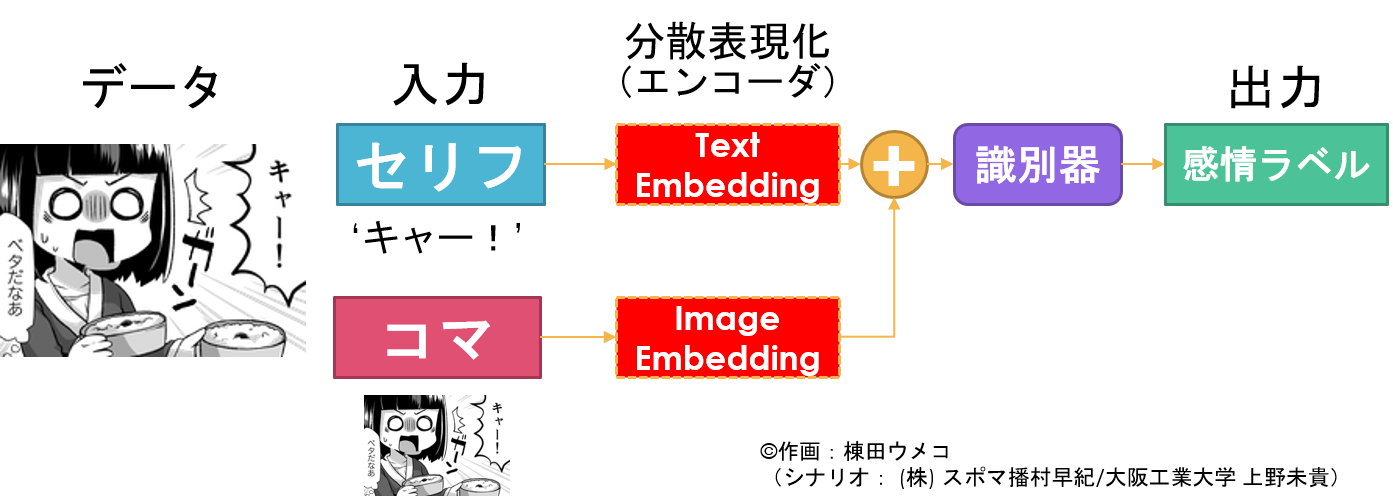
\includegraphics[scale=0.35]{teian.png}
  \caption{提案手法の概要}
  \label{fig:teian}
\end{figure}
%%%%%%%%%%%%%%%%%%%%%%%%%%%%%%
\section{実験}
本研究で用いるデータセットには 7 種類の感情ラベル(ニュートラル, 驚愕, 喜楽, 恐怖, 悲哀, 憤怒, 嫌悪)と, アノテーション不備によるラベル不明 (以下, ``UNK" とする) の全 8 種類
が含まれているが, データ数と解析の難しさの問題から, 喜楽のみを正例, その他の感情ラベルを負例とする 2 クラスに分類し, これを推定する.
\subsection{セリフ 1 文のみを入力とする感情推定}
...hottoSNS-BERT vs 京大 BERT
\subsection{マルチモーダルな感情推定の検討}
...hottoSNS-BERT vs 京大 BERT

%%%%%%%%%%%%%%%%%%%%%%%%%%%%%%
\section{まとめと今後の課題}
実験結果からマルチモーダルな感情推定の場合, ....

hottoSNS-BERTの方が...合理的...

今後の課題として, 現在の 4 コマ漫画ストーリーデータセットのみでの訓練・テストでは精度の向上が困難であることから, データセットの拡張が急がれる. この問題の解決策としては Manga109 やその他データセットを併用した半教師あり学習や, 人手による新しいデータの作成が挙げられる. データ作成の際にはオリジナルのデータからセリフ部分の文字を白抜きにしたコマの画像に対して, 物語の一貫性などの制約を設けた上で新たなセリフを作成し, 対応する感情ラベルを付与してもらうことで, このデータセットの ``作者による感情ラベルのアノテーション" という特徴を保ったままデータ拡張が可能であると考えられる. また, セリフから得たベクトルとコマの画像から得たベクトルの結合方法やネットワークの構造の最適化についても更なる工夫が必要である.


\bibliographystyle{jabbrvunsrt}
\bibliography{index_ja}
\end{document}
